%
%  outline latex source document for AV assignment 1.
%  use pdflatex to format this.
%
\documentclass[10pt,a4paper,oneclumn]{article}
\usepackage{amssymb,amsmath}            % if some maths is needed
\usepackage{graphicx}                   % if any images are to be included
% pick a different font if desired
\usepackage{times}

\title{Advanced Vision Assignment 2 Report}  % AILP: please use this title.
\author{Mindaugas Dabulskis, Marat Subkhankulov}                      % replace with name or exam number
\date{26th February 2013}                 % replace with actual date

\begin{document}

\maketitle  % insert title, author info
%
\section{Introduction}

This report describes the work done for the second assignment of the AV course.
The aim of the assignment was to track three coloured balls through a set of video frames.
The algorithm for ball detection and segmentation is discussed. 
The performance of the approach is evaluated using a gold standard.

\section{Algorithm and implementation}

In order to segment out the balls from the subject image (the current frame being considered), we removed background regions, and thresholded using values obtained from training data.

The following regions had to be removed from the image: 
\begin{enumerate}
\item Static background
\item Juggler's clothing
\item Juggler's hands
\item Juggler's face
\item Shadow caused by the juggler on the door
\end{enumerate}

To remove the above regions the following techniques were applied:
\begin{enumerate}
\item Average background subtraction
\item NRGB colourspace
\item HSV colourspace
\item Training samples based on ground truth
\end{enumerate}

\begin{center}
  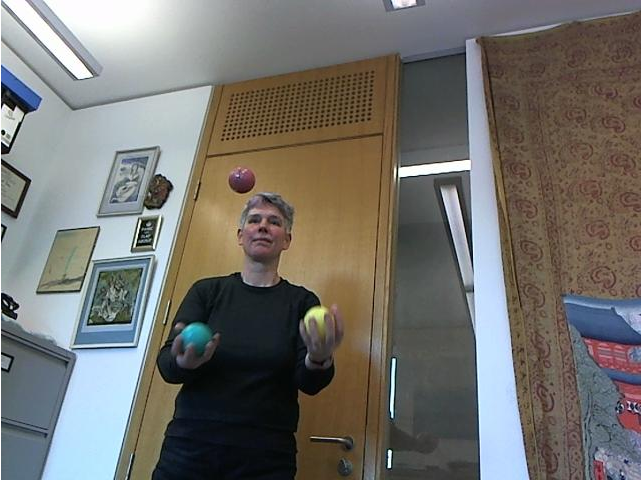
\includegraphics[width=6cm]{figures/original.png}
\end{center}

\subsection{Static background}

A picture of the empty room had been given, however when subtraction of the background from the subject image did not eliminate the shadow of the door, which had similar values to the yellow ball even in normalized RGB. Thus we obtained a mean of all the frames and used the resulting image as the background; By converting the subject and the new background images to N-RGB, subtracting and thresholding out the low brightness regions we obtained a mask which eliminated:
\begin{enumerate}
\item Static background
\item Shadow on the door
\item Juggler's face
\end{enumerate}

\begin{center}
  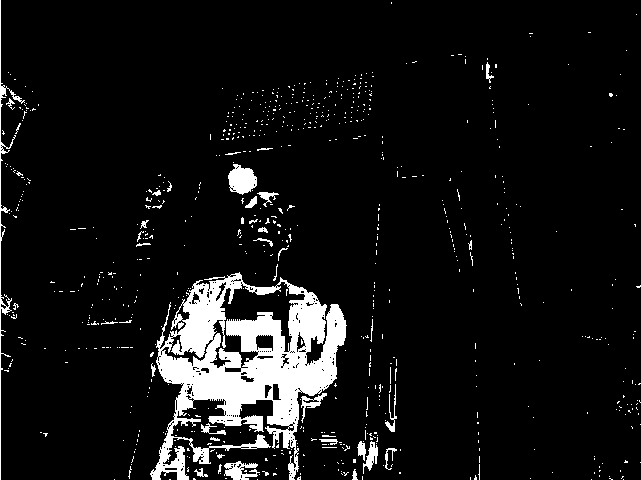
\includegraphics[width=6cm]{figures/avnrgbdifhsvmask.png}
\end{center}

\subsection{Slant normalisation}

Another algorithm.

\section{Experiments and results}

\section{Discussion and Conclusion}

\subsection{Formatting: tables}

An example of a table is shown as Table \ref{table1}. Somewhat 
different styles are allowed according to the type and purpose of the 
table. 

\begin{table} [t,h]
\caption{\label{table1} \textit{This is an example of a table.}}
\vspace{2mm}
\centerline{
\begin{tabular}{|c|c|}
\hline
ratio & decibels \\
\hline  \hline
1/1 & 0 \\
2/1 & $\approx 6$ \\
3.16 & 10 \\
10/1 & 20 \\ 
1/10 & -20 \\
100/1 & 40 \\
1000/1 & 60 \\
\hline
\end{tabular}}
\end{table}

To include text without formatting, use this
(scriptsize uses a significantly smaller font,
intermediate sizes are footnotesize and small):
{\scriptsize
\begin{verbatim}
I\O     1     2     3     4     5     6     7     8     9    10
  1  71.2   8.8   1.2   0.0   2.5   3.8   7.5   0.0   5.0   0.0
  2   0.0  87.5   1.2   0.0   2.5   2.5   0.0   5.0   0.0   1.2
  3   0.0   0.0  67.5   5.0   1.2  11.2   3.8   7.5   3.8   0.0
  4   0.0   0.0   1.2  62.5   3.8  22.5   0.0   6.2   2.5   1.2
  5   0.0   2.5   0.0   0.0  76.2   0.0   1.2   6.2   0.0  13.8
  6   5.0   1.2   6.2  21.2   5.0  47.5   1.2   5.0   1.2   6.2
  7  17.5   6.2   3.8   0.0   5.0   0.0  57.5   0.0  10.0   0.0
  8   0.0   0.0   2.5   1.2   8.8   0.0   0.0  73.8   2.5  11.2
  9  11.2   0.0   2.5   8.8   2.5   3.8   5.0   2.5  61.3   2.5
 10   1.2   0.0   0.0   2.5  20.0   0.0   0.0  12.5   0.0  63.7
\end{verbatim}
}

If you want to use both columns, put it in a figure*:
(figure* uses both columns, figure just 1):
it is likely to float away to an unexpecte place, though.
\begin{figure*}[h]
  \centering
{\small
\begin{verbatim}
I\O     1     2     3     4     5     6     7     8     9    10
  1  71.2   8.8   1.2   0.0   2.5   3.8   7.5   0.0   5.0   0.0
  2   0.0  87.5   1.2   0.0   2.5   2.5   0.0   5.0   0.0   1.2
  3   0.0   0.0  67.5   5.0   1.2  11.2   3.8   7.5   3.8   0.0
  4   0.0   0.0   1.2  62.5   3.8  22.5   0.0   6.2   2.5   1.2
  5   0.0   2.5   0.0   0.0  76.2   0.0   1.2   6.2   0.0  13.8
  6   5.0   1.2   6.2  21.2   5.0  47.5   1.2   5.0   1.2   6.2
  7  17.5   6.2   3.8   0.0   5.0   0.0  57.5   0.0  10.0   0.0
  8   0.0   0.0   2.5   1.2   8.8   0.0   0.0  73.8   2.5  11.2
  9  11.2   0.0   2.5   8.8   2.5   3.8   5.0   2.5  61.3   2.5
 10   1.2   0.0   0.0   2.5  20.0   0.0   0.0  12.5   0.0  63.7
\end{verbatim}
}

  \caption{Confusion Matrix}
  
\end{figure*}

\subsection{Maths, if needed}

%
%\vspace{-3mm}
\begin{equation}
x(t) = s(f_\omega(t))
\label{eq1}
\end{equation}
where \(f_\omega(t)\) is a special warping function
\begin{equation}
f_\omega(t)=\frac{1}{2\pi j}\oint_C \frac{\nu^{-1k}d\nu}
{(1-\beta\nu^{-1})(\nu^{-1}-\beta)}
\label{eq2}
\end{equation}
A residue theorem states that
\begin{equation}
\oint_C F(z)dz=2 \pi j \sum_k Res[F(z),p_k]
\label{eq3}
\end{equation}
Applying (\ref{eq3}) to (\ref{eq1}), 
it is straightforward to see that
\begin{equation}
1 + 1 = \pi
\label{eq4}
\end{equation}

And here is an included image (png and pdf formats are allowed).

\subsection{References}

References should be numbered in order of appearance, 
for example \cite{ES1}, \cite{ES2}, and \cite{ES3}. 
You \emph{can} use \texttt{bibtex} to prepare references,
or do it by hand if there are very few.

%
\bibliographystyle{IEEEtran}
\begin{thebibliography}{10}
\bibitem[1]{ES1} Smith, J. O. and Abel, J. S., 
``Bark and {ERB} Bilinear Transforms'', 
IEEE Trans. Speech and Audio Proc., 7(6):697--708, 1999.  
\bibitem[2]{ES2} Lee, K.-F., Automatic Speech Recognition: 
The Development of the 
SPHINX SYSTEM, Kluwer Academic Publishers, Boston, 1989.
\bibitem[3]{ES3} Rudnicky, A. I., Polifroni, Thayer, E. H.,
 and Brennan, R. A.  
"Interactive problem solving with speech", J. Acoust. Soc. Amer., 
Vol. 84, 1988, p S213(A).
\end{thebibliography}
\end{document}
